\chapter{User Guide} \label{Guide}
% You must provide an adequate user guide for your software. The guide should provide easily understood instructions on how to use your software. A particularly useful approach is to treat the user guide as a walk-through of a typical session, or set of sessions, which collectively display all of the features of your package. Technical details of how the package works are rarely required. Keep the guide concise and simple. The extensive use of diagrams, illustrating the package in action, can often be particularly helpful. The user guide is sometimes included as a chapter in the main body of the report, but is often better included in an appendix to the main report.

\section{Opening Godot}

To run the projects in the .zip file, extract the projects into one folder. Then open Godot 4 (all projects in the source code listings folder are Godot 4 projects, \textbf{not} Godot 3 projects). When you start Godot for the first time, the project manager should be completely empty, without any projects, as described in Figure \ref{fig:godot1}. Projects have to be imported either one-by-one (by clicking ``Import" and going to the relevant project and opening it) or by clicking "Scan", then going to a folder of Godot projects and selecting it. The projects can then be opened in the project manager and edited as needed in Godot. Click ``Scan", then go to the folder where you extracted the projects, then click the ``Select Current Folder" button, as shown in Figure \ref{fig:godot2}, and all the projects should show up in the editor, as shown in Figure \ref{fig:godot3}. You can then double click on any one project (or click on it once and click the ``Edit" button) to open it in the Godot editor, an example of which is shown in Figure \ref{fig:godot4}. Alternatively, to run the project itself without opening the editor, using the currently saved values for exported script variables where appropriate, click on the project \textit{once} and click the ``Run" button.

\begin{figure}[H]
    \centering
    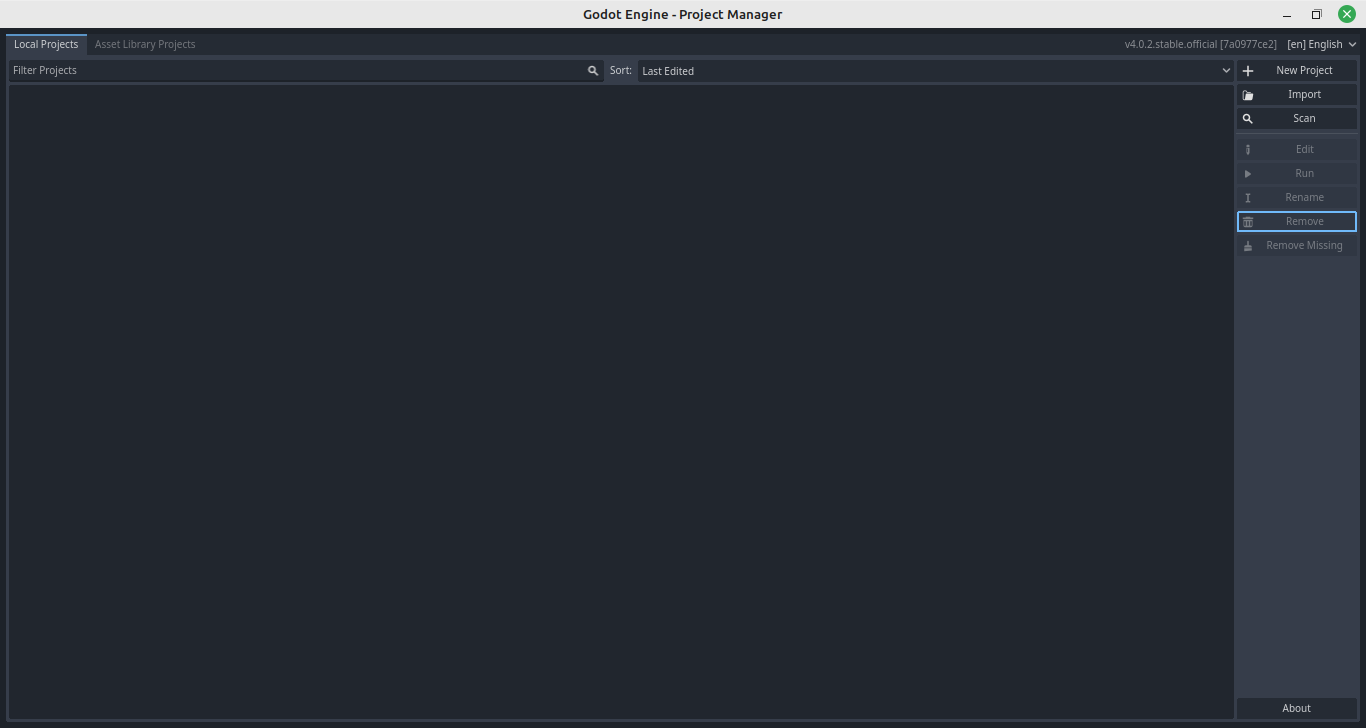
\includegraphics[width=\textwidth]{Images/open_godot.png}
    \caption{The Godot editor, when it is opened for the first time, does not show any projects in the editor (the Steam version bundles several example projects). Projects need to be imported either one-by-one or by scanning a folder of Godot projects.}
    \label{fig:godot1}
\end{figure}

\begin{figure}[H]
    \centering
    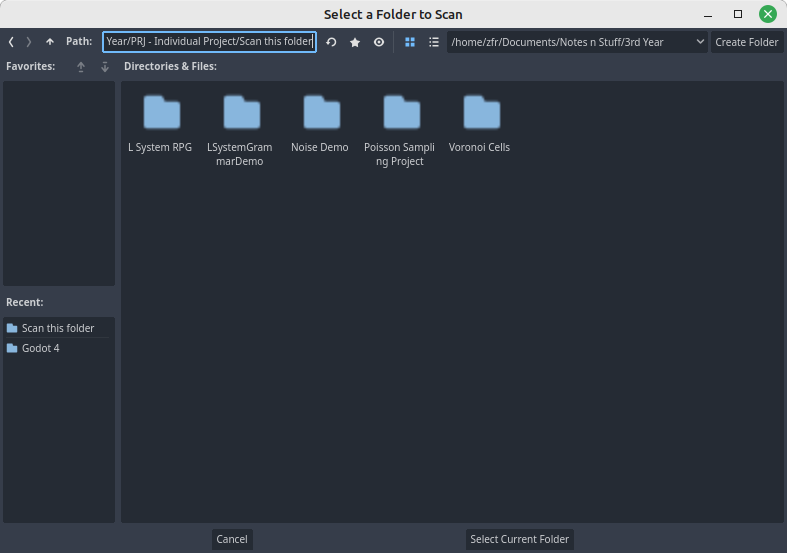
\includegraphics[width=\textwidth]{Images/scan-folder.png}
    \caption{You can click the "Scan" button in the project manager (in Figure \ref{fig:godot1}), then go to the relevant folder where your project are in Godot's built-in file explorer. Here, I have extracted my artefacts into a separate folder called ``Scan this folder" as an example.}
    \label{fig:godot2}
\end{figure}

\begin{figure}[H]
    \centering
    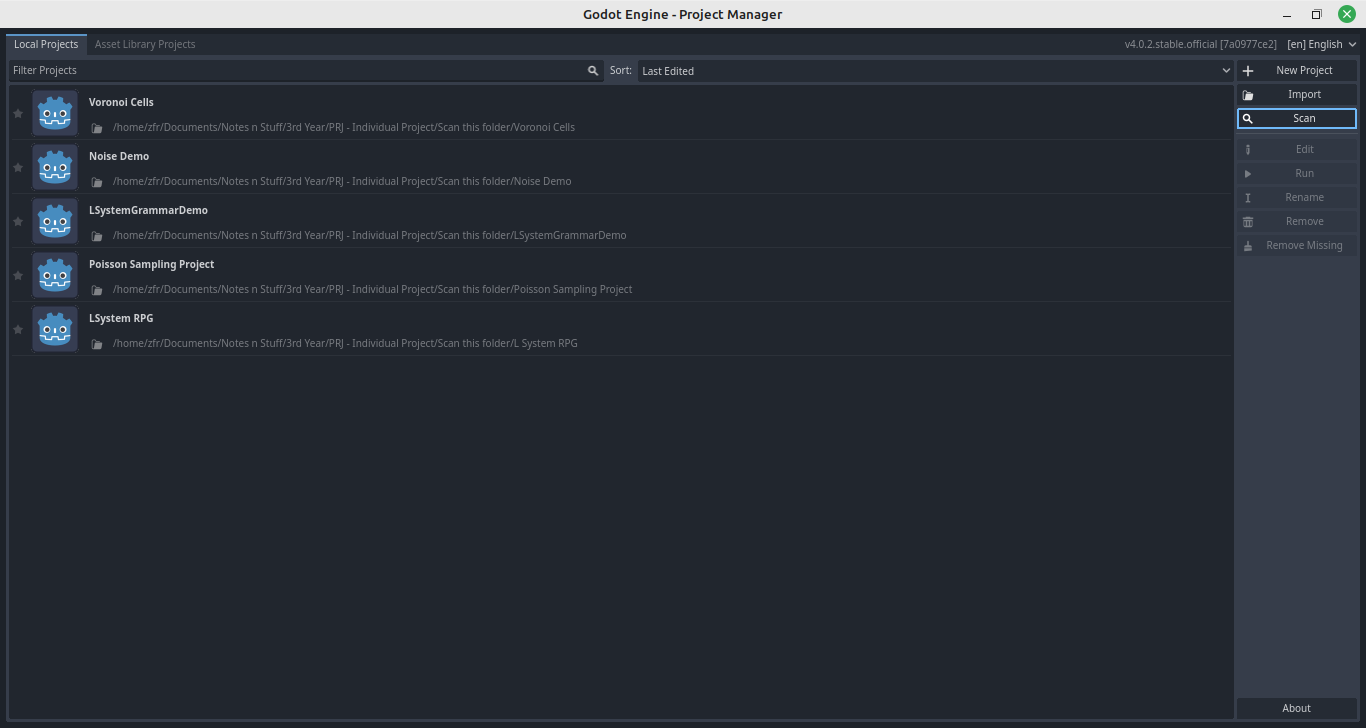
\includegraphics[width=\textwidth]{Images/projects-scanned.png}
    \caption{Once some Godot projects have been imported into the project manager, you should be able to easily view the list and double-click on any one of the projects to edit them, which will open the editor after closing the project manager. You could also click the ``Edit" button, or click ``Run" to run the game without having to open the editor itself.}
    \label{fig:godot3}
\end{figure}

\begin{figure}[H]
    \centering
    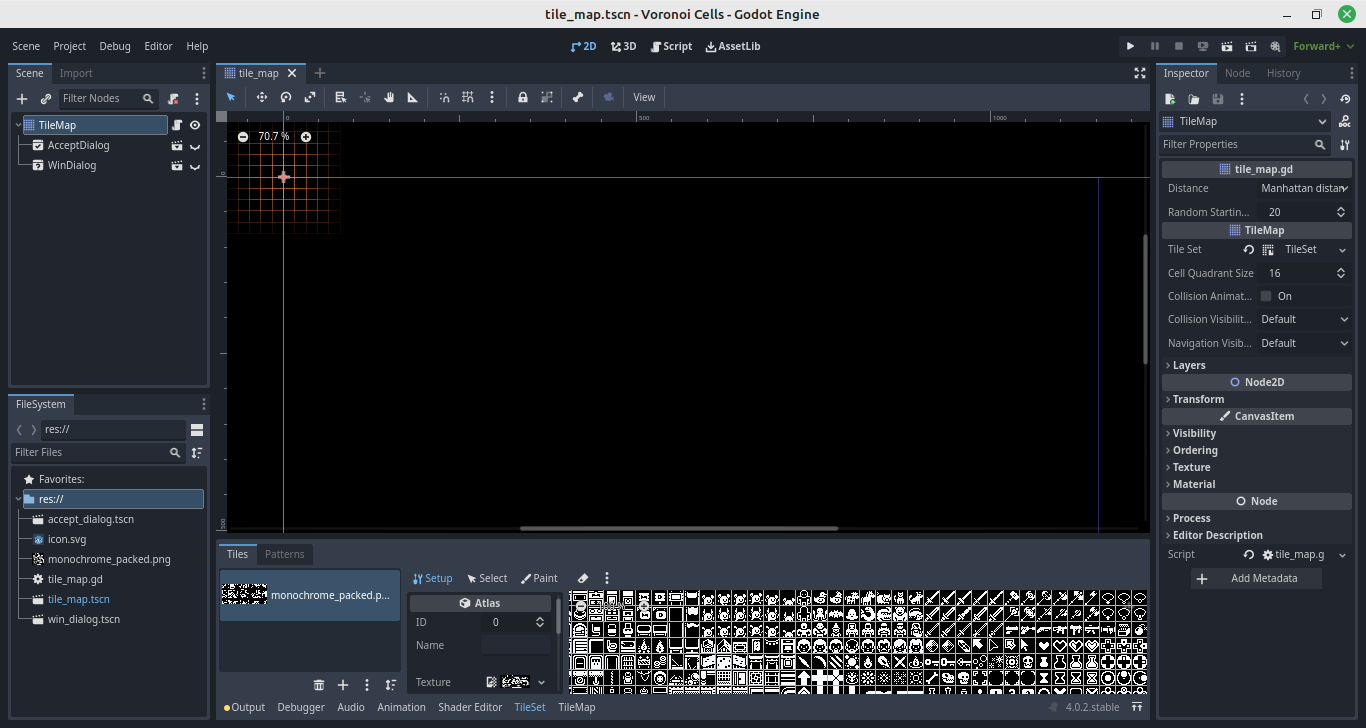
\includegraphics[width=\textwidth]{Images/godot-editor.png}
    \caption{The Godot editor open with the Voronoi cells project as an example. A visual description of the editor's contents is in chapter \ref{editor}.}
    \label{fig:godot4}
\end{figure}

\section{The Godot Editor} \label{editor}

As you open up the Godot editor, you will see the main scene view in the center, as shown in Figure \ref{fig:godot4}, using the Voronoi cells implementation as an example. The left-hand side shows the scene tree at the top, and the file system (from the root folder of the project) at the bottom. Meanwhile, the right hand side shows the currently selected node's export variables, \textit{including the custom export variables} defined in the node's script file, and two other tabs, ``Node" (which shows a list of signals for the scene that could be called in a script) and ``History" (which shows the sequence of recent actions performed on the scene during the current session). Above this is also a set of buttons which can be used for playing the project and/or the current scene. I go over how to run the current project in chapter \ref{runproject}.

\section{Custom Export Variables} 

When you click on some of the scenes in the projects, there may be some "exported" variables from scripts that are visible to you in the editor (examples include the "Distance" and "Random Starting Points" variables in the Voronoi Cells project). You can hover over the variable names in the editor and it will show a brief description of what the variable correlates to in the script. I go over the different export variables across all of my artefacts in this section.

\subsection{Lindenmayer System}

\begin{itemize}
    \item 
\end{itemize}

\subsection{Perlin/Simplex Noise}

\begin{itemize}
    \item 
\end{itemize}

\subsection{Poisson Disk Sampling}

\begin{itemize}
    \item 
\end{itemize}

\subsection{Voronoï Cells}

\begin{itemize}
    \item 
\end{itemize}

\subsection{The Basic L-System Demo Used to Create the Screenshots in Chapter \ref{alglsys}}

There is only one export variable for this: ``choices", which allows you to choose which one of the three provided rulesets to use. ``choices" is the default ruleset, and either ``deterministic" or ``basic" can be chosen.

\section{Running the Godot Projects} \label{runproject}

To \textit{run} the current project in the Godot editor, go to the bar above the Inspector, Node and History tabs on the right-hand side. You will find a \faPlay{} button which will play the main scene of the project (in my artefacts, the main scenes have already been set; if it were not already set, you would have been asked to set one).
